\documentclass{article}
\usepackage{../../../../TechDocs/LatexStyles/standard-4}
\newcommand{\x}{x(\hat{x})}
\begin{document}

\section{Test For The Conservation of LDFEM Discretized Hydrodynamics Equations - No Energy Coupling}
The compressible conservation mass and momentum equations are shown below,
\begin{align}
\label{eq::ConsMass}
&\frac{\pd}{\pd x}\left( \rho(x) u(x) \right) = S_m,\\[5pt]
\label{eq::ConsMomen}
&\frac{\pd}{\pd x}\left( \rho(x) u(x)^2 + P(x) \right) = S_\rho.
\end{align}

For the purposes of the following tests, we will assume the following manufactured solutions,
\begin{align}
\label{eq::MMS-Velocity}
u(x) &= 2.0 - x,\\[5pt]
\label{eq::MMS-Density}
\rho(x) &= 1.0 + x.
\end{align}

% ==============================
%       Conservation of Mass
% ==============================
\subsection{Conservation of Mass}
Discretizing the conservation of mass (Equation \ref{eq::ConsMass}) using discontinuous finite elements results in the following,
\begin{align}
\label{eq::LDFEM-MassLHS-1}
&\frac{u_{i,1}\rho_{i,1}}{3} + \frac{u_{i,1}\rho_{i,2}}{6} + \frac{u_{i,2}\rho_{i,1}}{6} + \frac{u_{i,2}\rho_{i,2}}{3} = f_{m;i,1},\\[5pt]
\label{eq::LDFEM-MassLHS-2}
-&\frac{u_{i,1}\rho_{i,1}}{3} - \frac{u_{i,1}\rho_{i,2}}{6} - \frac{u_{i,2}\rho_{i,1}}{6} - \frac{u_{i,2}\rho_{i,2}}{3} + u_{i,2}\rho_{i,2} = f_{m;i,2},
\end{align}
where,
\begin{align}
\label{eq::LDFEM-MassRHS-1}
f_{m;i,1} &= u_{i-1,2}\rho_{i-1,2} + \left( \frac{d}{dx}\rho(\x) u(\x) + \rho(\x)\frac{d}{dx}u(\x) \right),\\[5pt]
\label{eq::LDFEM-MassRHS-2}
f_{m;i,2} &= \left( \frac{d}{dx}\rho(\x)u(\x) + \rho(\x)\frac{d}{dx}u(\x) \right).
\end{align}

We test for conservativeness by inserting Equations \ref{eq::MMS-Velocity} and \ref{eq::MMS-Density} into Equations \ref{eq::LDFEM-MassLHS-1} through \ref{eq::LDFEM-MassRHS-2}. With the assumed analytic solutions, we should observe that the residual of Equations \ref{eq::LDFEM-MassLHS-1} and \ref{eq::LDFEM-MassLHS-2} are near zero. As an example, we show how the residual is computed for Equation \ref{eq::LDFEM-MassLHS-1},
\begin{equation}
    \label{eq::Residual}
    \text{Abs. Diff.} = \lvert \left( \frac{u_{i,1}\rho_{i,1}}{3} + \frac{u_{i,1}\rho_{i,2}}{6} + \frac{u_{i,2}\rho_{i,1}}{6} + \frac{u_{i,2}\rho_{i,2}}{3} \right) - f_{m;i,1} \rvert.
\end{equation}
Note, an analogous norm is defined for Equation \ref{eq::LDFEM-MassLHS-2}. Figures \ref{fig::Mass-1} and \ref{fig::Mass-2} show the that the discretized equations (Equations \ref{eq::LDFEM-MassLHS-1} and \ref{eq::LDFEM-MassLHS-2}) are conservative.
\begin{figure}[h!]
\centering
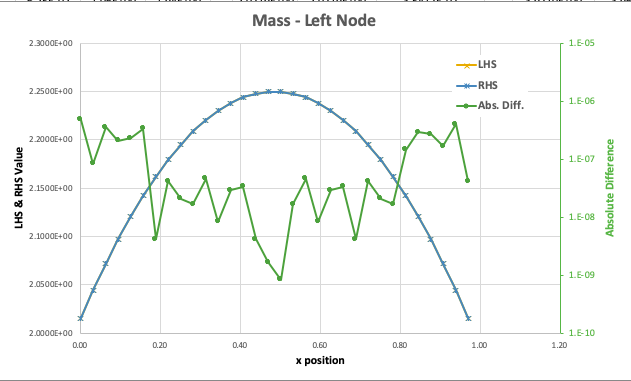
\includegraphics[scale=0.4]{./figures/Mass_1}
\caption{Test for conservation of discretized mass equations - left node.}
\label{fig::Mass-1}
\end{figure}
\begin{figure}[h!]
\centering
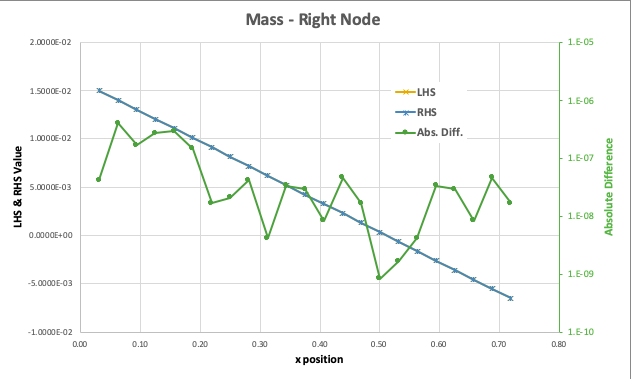
\includegraphics[scale=0.4]{./figures/Mass_2}
\caption{Test for conservation of discretized mass equations - right node.}
\label{fig::Mass-2}
\end{figure}


% ==============================
%       Conservation of Momentum
% ==============================
\subsection{Conservation of Momentum}
Discretizing the conservation of momentum (Equation \ref{eq::ConsMomen}) using discontinuous finite elements results in the following,
\begin{align}
\label{eq::LDFEM-MomenLHS-1}
&\frac{\rho_{i,1}u_{i,1}^2}{4} + \frac{\rho_{i,2}u_{i,1}^2}{12} + \frac{\rho_{i,1}u_{i,1}u_{i,2}}{6} + \frac{\rho_{i,2}u_{i,1}u_{i,2}}{6} + \frac{\rho_{i,1}u_{i,2}^2}{12} + \frac{\rho_{i,2}u_{i,2}^2}{4} = f_{\rho;i,1},\\[5pt]
\label{eq::LDFEM-MomenLHS-2}
-&\frac{\rho_{i,1}u_{i,1}^2}{4} - \frac{\rho_{i,2}u_{i,1}^2}{12} - \frac{\rho_{i,1}u_{i,1}u_{i,2}}{6} - \frac{\rho_{i,2}u_{i,1}u_{i,2}}{6} - \frac{\rho_{i,1}u_{i,2}^2}{12} - \frac{\rho_{i,2}u_{i,2}^2}{4} + \rho_{i,2}u_{i,2}^2 = f_{\rho;i,2},
\end{align}
where,
\begin{align}
\label{eq::LDFEM-MomenRHS-1}
f_{\rho;i,1} &= -\frac{d}{dx}P_{i,1}(\x) + \rho_{i-1,2}u_{i-1,2}^2 + \left( \rho(\x)2u(\x)\frac{d}{dx}u(\x) + \frac{d}{dx}\rho(\x)u(\x)^2 \right),\\[5pt]
\label{eq::LDFEM-MomenRHS-2}
f_{\rho;i,2} &= -\frac{d}{dx}P_{i,2}(\x) + \left( \rho(\x)2u(\x)\frac{d}{dx}u(\x) + \frac{d}{dx}\rho(\x)u(\x)^2 \right).
\end{align}

As before, we test for conservativeness by inserting Equations \ref{eq::MMS-Velocity} and \ref{eq::MMS-Density} into Equations \ref{eq::LDFEM-MomenLHS-1} through \ref{eq::LDFEM-MomenRHS-2}. Again, we should observe that the residuals of Equations \ref{eq::LDFEM-MomenLHS-1} and \ref{eq::LDFEM-MomenLHS-2} should be nearly zero. Residuals are computed using analogous norms to Equation \ref{eq::Residual}. Figures \ref{fig::Momen-1} and \ref{fig::Momen-2} show the that the discretized equations for Equation \ref{eq::ConsMomen} are \textbf{not} conservative.
\begin{figure}[h!]
\centering
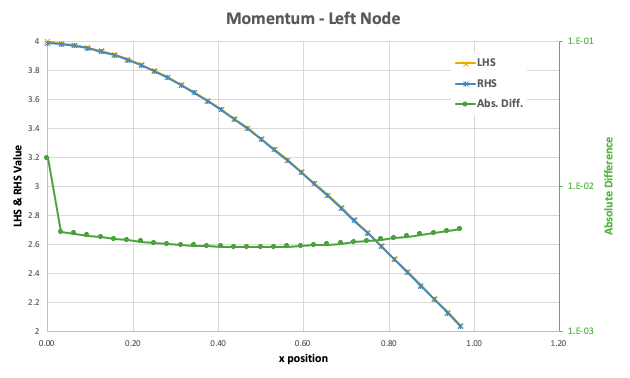
\includegraphics[scale=0.4]{./figures/Momen_1}
\caption{Test for conservation of discretized momentum equations - left node.}
\label{fig::Momen-1}
\end{figure}
\begin{figure}[h!]
\centering
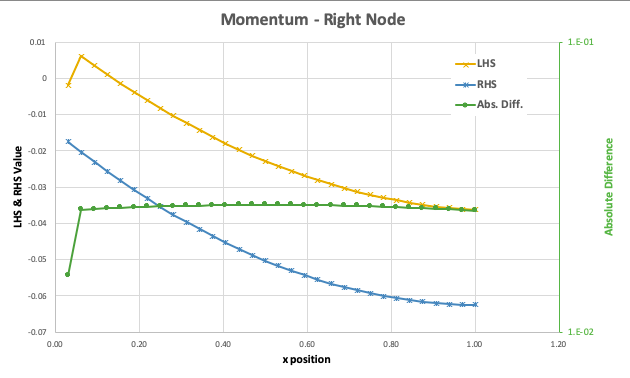
\includegraphics[scale=0.4]{./figures/Momen_2}
\caption{Test for conservation of discretized momentum equations - right node.}
\label{fig::Momen-2}
\end{figure}





\end{document}